\section{Aufbau und Durchführung}
\subsection{Aufbau}
\label{sec:Aufbau}

\subsubsection{Optischer Aufbau}

Der gesamte Versuchsaufbau ist in Abbildung \ref{abb:2} dargestellt.
\begin{figure}
  \centering
  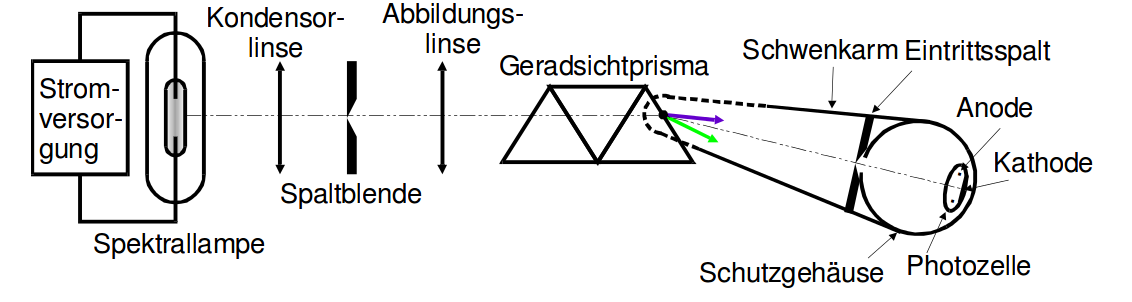
\includegraphics[height=4cm]{ressources/aufbau_2.png}
  \caption{Gesamte Übersicht über den verwendeten Versuchsaufbau. \cite{skript}}
  \label{abb:2}
\end{figure}

Die Spektrallampe emittiert Licht mit diskreten Wellenlängen. Dieses wird unter Verwendung einer Kondensorlinse, einer Spaltblende sowie einer Abbildungslinse auf ein Prisma fokussiert und abgebildet.
Dieses Prisma bricht das Licht, so dass dieses auf Grund der optischen Dispersion für jede Wellenlänge unterschiedlich stark gebrochen wird.
Der Öffnungsspalt der Photozelle wird nun so ausgerichtet, dass das Licht der zu messenden Wellenlänge auf die Kathode einfällt.

\subsubsection{Bestimmung der Photonenenergie mithilfe der Gegenfeldmethode}

Um eine quantitative Aussage über die kinetische Energie der Elektronen, welche aus der Photokathode gelöst werden, treffen zu können, wird der in Abbildung \ref{abb:3} dargestellte Aufbau verwendet.

\begin{figure}
  \centering
  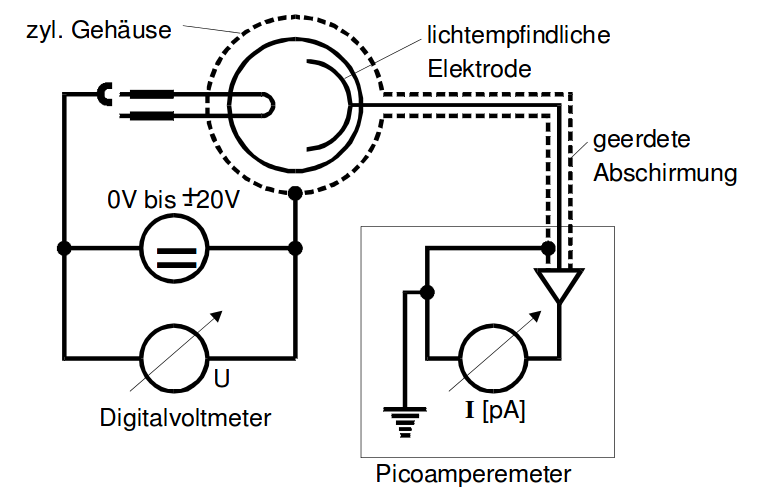
\includegraphics[height=6cm]{ressources/aufbau_3.png}
  \caption{Aufbau der Photozelle zur Verwendung der Gegenfeldmethode. \cite{skript}}
  \label{abb:3}
\end{figure}

Zwischen der Photokathode und einer Anode kann eine Spannung $U$ angelegt werden, die je nach Polung als Bremsspannung oder Beschleunigungsspannung für die Elektronen dienen kann.
Verfügen die Elektronen über eine ausreichende kinetische Energie um die Gegenspannung überwinden zu können, erreichen diese die Anode.
Solange dies erfüllt ist, kann mithilfe eines Picoamperemeters ein geringer Strom zwischen Kathode und Anode gemessen werden.
